\section{C/C++ Binding}
\label{sec:C}

COMPSs provides a binding for C and C++ applications. The new C++ version in the current release 
comes with support for objects as task parameters and the use of class methods as tasks.

\subsection{Programming Model}

\subsubsection{Task Selection}
As in Java the user has to provide a task selection by means of an interface. In this case 
the interface file has the same name as the main application file plus the suffix ``idl'', 
i.e. Matmul.idl, where the main file is called Matmul.cc.

\begin{lstlisting}[language=C++]
interface Matmul
{
      // C functions
      void initMatrix(inout Matrix matrix,
                      in int mSize,
                      in int nSize,
                      in double val);
                      
      void multiplyBlocks(inout Block block1,
                          inout Block block2,
                          inout Block block3);
};
\end{lstlisting}
%OLD                          
%      // C++ class methods
%      void Block::multiply(in Block block1,
%                           in Block block2);
%                           
%      static Matrix Matrix::init(in int mSize,
%                                 in int bSize,
%                                 in double val);
%};
%\end{lstlisting}

The syntax of the interface file is shown in the previous code. Tasks can be declared as classic 
C function prototypes, this allow to keep the compatibility with standard C applications. 
In the example, initMatrix and multiplyBlocks are functions declared using its prototype, 
like in a C header file, but this code is C++ as they have objects as parameters (objects of 
type Matrix, or Block).

%A class method can be also a task, and it is declared using its signature. In the example, 
%Block::multiply and Matrix::init are class methods. In this example, C functions encapsulates 
%object method calls, as we will see later.

The grammar for the interface file is:

\begin{lstlisting}[language=bash]
["static"] return-type task-name ( parameter {, parameter }* );

return-type = "void" | type

ask-name = <qualified name of the function or method>

parameter = direction type parameter-name

direction = "in" | "out" | "inout"

type = "char" | "int" | "short" | "long" | "float" | "double" | "boolean" |
       "char[<size>]" | "int[<size>]" | "short[<size>]" | "long[<size>]" |
       "float[<size>]" | "double[<size>]" | "string" | "File" | class-name

class-name = <qualified name of the class>
\end{lstlisting}

% The following text  is not true in current version       
%\subsubsection{Value return} 
%The binding allows returning a value (void, int, long, float, etc.) from a 
%function or method. In C/C++ the default policy is to make a copy of the value or object when it is returned [A = foo();], 
%and this copy (A) is a new position in memory whom reference or address is not possible to know before 
%the return statement. As the COMPSs runtime cannot know such reference before returning from the task execution (foo) it must do a 
%synchronization before the return statement for the correct value to be copied when returning. 
%This is called an explicit synchronization.

%Alternatively, the return of a value or an object can be done also by mean of an out or inout parameter, 
%and no explicit synchronization is needed because the reference is passed to the binding in this case 
%using the \& operator [foo(\&A);].

\subsubsection{Main Program}
The next listing includes an example of matrix multiplication written in C++.

\begin{lstlisting}[language=C++]
#include %*{\bf "Matmul.h" }*)
#include "Matrix.h"
#include "Block.h"
int N; //MSIZE
int M; //BSIZE
double val;
int main(int argc, char **argv)
{
      Matrix A;
      Matrix B;
      Matrix C;

       N = atoi(argv[1]);
       M = atoi(argv[2]);
      val = atof(argv[3]);

      %*{\bf compss\_on(); }*)

      A = Matrix::init(N,M,val);

      initMatrix(&B,N,M,val);
      initMatrix(&C,N,M,0.0);

      cout << "Waiting for initialization...\n";

      %*{\bf compss\_wait\_on(B); }*)
      %*{\bf compss\_wait\_on(C); }*)

      cout << "Initialization ends...\n";
 
      C.multiply(A, B);

      %*{\bf compss\_off(); }*)
      return 0;
}
\end{lstlisting}

The developer has to take into account the following rules:
\begin{enumerate}
 \item A header file with the same name as the main file must be included, in this case {\bf Matmul.h}. 
       This header file is automatically generated by the binding and it contains other includes and 
        type-definitions that are required.
 \item A call to the {\bf compss\_on} binding function is required to turn on the COMPSs runtime.
 \item As in C language, out or inout parameters should be passed by reference by means of the ``{\bf \&}'' 
       operator before the parameter name.
 \item Synchronization on a parameter can be done calling the {\bf compss\_wait\_on} binding function. 
       The argument of this function must be the variable or object we want to synchronize.
 \item There is an {\bf implicit synchronization} in the init method of Matrix. It is not possible to 
       know the address of ``A'' before exiting the method call and due to this it is necessary to synchronize 
       before for the copy of the returned value into ``A'' for it to be correct.
 \item A call to the {\bf compss\_off} binding function is required to turn off the COMPSs runtime.
\end{enumerate}


\subsubsection{Binding API}
Besides the aforementioned {\bf compss\_on}, {\bf compss\_off} and {\bf compss\_wait\_on} functions, the C/C++ main program can make use of a variety of other API calls to better manage the synchronization of data generated by tasks. These calls are as follows:

\begin{itemize}
 \item {\it void compss\_ifstream(char * filename, ifstream }\& {\it ifs)}: given an uninitialized input stream {\it ifs} and a file {\it filename}, this function will synchronize the content of the file and initialize {\it ifs} to read from it.
 
 \item {\it void compss\_ofstream(char * filename, ofstream }\& {\it ofs)}: behaves the same way as {\it compss\_ifstream}, but in this case the opened stream is an output stream, meaning it will be used to write to the file.

 \item {\it FILE* compss\_fopen(char * file\_name, char * mode)}: similar to the C/C++ {\it fopen} call. Synchronizes with the last version of file {\it file\_name} and returns the FILE* pointer to further reference it. As the mode parameter it takes the same that can be used in {\it fopen} ({\it r, w, a, r+, w+} and {\it a+}). 
       
 \item {\it void compss\_wait\_on(T* }\& {\it obj) or T compss\_wait\_on(T }\& {\it obj)}: synchronizes for the last version of object obj, meaning that the execution will stop until the value of {\it obj} up to that point of the code is received (and thus all tasks that can modify it have ended).
 
 \item {\it void compss\_delete\_file(char * file\_name)}: makes an asynchronous delete of file {\it filename}. When all previous tasks have finished updating the file, it is deleted.
 
 \item {\it void compss\_delete\_object(T* }\& {\it obj)}: makes an asynchronous delete of an object. When all previous tasks have finished updating the object, it is deleted.
       
 \item {\it void compss\_barrier()}: similarly to the Python binding, performs an explicit synchronization without a return. When a {\it compss\_barrier} is encountered, the execution will not continue until all the tasks submitted before the {\it compss\_barrier} have finished.
\end{itemize}


\subsubsection{Functions file}
\label{sec:functionsfile}
The implementation of the tasks in a C or C++ program has to be provided in a functions file. 
Its name must be the same as the main file followed by the suffix ``-functions''. In our case Matmul-functions.cc.

\begin{lstlisting}[language=C++]
#include "Matmul.h"
#include "Matrix.h"
#include "Block.h"

void initMatrix(Matrix *matrix,int mSize,int nSize,double val){
     *matrix = Matrix::init(mSize, nSize, val);
}

void multiplyBlocks(Block *block1,Block *block2,Block *block3){
     block1->multiply(*block2, *block3);
}
\end{lstlisting}

In the previous code, class methods have been encapsulated inside a function. 
This is useful when the class method returns an object or a value and we want to avoid the explicit 
synchronization when returning from the method.

\subsubsection{Additional source files}
\label{sec:additionalsources}

Other source files needed by the user application must be placed under the directory ``{\bf src}''.
In this directory the programmer must provide a {\bf Makefile} that compiles such source files in the proper way. 
When the binding compiles the whole application it will enter into the src directory and execute the Makefile.
 
It generates two libraries, one for the master application and another for the worker application. 
The directive COMPSS\_MASTER or COMPSS\_WORKER must be used in order to compile the source files for each type of library. 
Both libraries will be copied into the lib directory where the binding will look for them when generating the master and worker applications.

\subsubsection{Class Serialization}
In case of using an object as method parameter, as callee or as return of a call to a function, the object has to be serialized. The serialization method has to be provided inline in the header file of the object's class by means of the ``{\bf boost}'' library. The next listing contains an example of serialization for two objects of the Block class.

\begin{lstlisting}[language=C++]
#ifndef BLOCK_H
#define BLOCK_H

#include    <vector>
#include    <boost/archive/text_iarchive.hpp>
#include    <boost/archive/text_oarchive.hpp>
#include    <boost/serialization/serialization.hpp>
#include    <boost/serialization/access.hpp>
#include    <boost/serialization/vector.hpp>

using namespace std;
using namespace boost;
using namespace serialization;

class Block {
public:
    Block(){};
    Block(int bSize);   
    static Block *init(int bSize, double initVal);
    void multiply(Block block1, Block block2);    
    void print();

private:
    int M;
    std::vector< std::vector< double > > data;
        
    %*{\bf friend class::serialization::access; }*)
    %*{\bf template$<$class Archive$>$ }*)
    %*{\bf void serialize(Archive \& ar, const unsigned int version) \{ }*)
        %*{\bf ar \& M; }*)
        %*{\bf ar \& data; }*)
    %*{\bf \} }*)
};
#endif
\end{lstlisting}

For more information about serialization using ``boost'' visit the related documentation at \url{www.boost.org}.


\subsubsection{Method - Task}

A task can be a C++ class method. A method can return a value, modify the \textit{this} object, or modify a parameter.

If the method has a return value there will be an implicit synchronization before exit the method, 
but for the \textit{this} object and parameters the synchronization can be done later after the method has finished.

This is because the \textit{this} object and the parameters can be accessed inside and outside the method, but for the 
variable where the returned value is copied to, it can’t be known inside the method.

\begin{lstlisting}[language=C++]
#include "Block.h"

Block::Block(int bSize) {
       M = bSize;
       data.resize(M);
       for (int i=0; i<M; i++) {
              data[i].resize(M);
       }
}

Block *Block::init(int bSize, double initVal) {
       Block *block = new Block(bSize);
       for (int i=0; i<bSize; i++) {
              for (int j=0; j<bSize; j++) {
                     block->data[i][j] = initVal;
              }
       }
       return block;
}

#ifdef COMPSS_WORKER

void Block::multiply(Block block1, Block block2) {
       for (int i=0; i<M; i++) {
              for (int j=0; j<M; j++) {
                     for (int k=0; k<M; k++) {
                            data[i][j] += block1.data[i][k] * block2.data[k][j];
                     }
              }
       }
       this->print();
}

#endif

void Block::print() {
       for (int i=0; i<M; i++) {
              for (int j=0; j<M; j++) {
                     cout << data[i][j] << " ";
              }
              cout << "\r\n";
       }
}
\end{lstlisting}

\subsubsection{Task Constraints}
The C/C++ binding also supports the definition of task constraints. The task definition specified in the IDL file must be decorated/annotated with the \textit{@Constraints}. 
Below, you can find and example of how to define a task with a constraint of using 4 cores. The list of constraints which can be defined for a task can be found in Section~\ref{sec:Constraints}

\begin{lstlisting}[language=C++]
interface Matmul
{
      @Constraints(ComputingUnits = 4
      void multiplyBlocks(inout Block block1,
                          in Block block2,
                          in Block block3);
                          
};
\end{lstlisting}


\subsubsection{Task Versions}
Another COMPSs functionality supported in the C/C++ binding is the definition of different versions for a tasks. 
The following code shows an IDL file where a function has two implementations, with their corresponding constraints. 
It show an example where the \textit{multiplyBlocks\_GPU} is defined as a implementation of \textit{multiplyBlocks} using the annotation/decoration \textit{@Implements}. 
It also shows how to set a processor constraint which requires a GPU processor and a CPU core for managing the offloading of the computation to the GPU. 
\begin{lstlisting}[language=C++]
interface Matmul
{
        @Constraints(ComputingUnits=4);
        void multiplyBlocks(inout Block block1, 
                            in Block block2,
                            in Block block3);

        // GPU implementation 
        @Constraints(processors={
               @Processor(ProcessorType=CPU, ComputingUnits=1)});
               @Processor(ProcessorType=GPU, ComputingUnits=1)});
        @Implements(multiplyBlocks);
        void multiplyBlocks_GPU(inout Block block1,
                                in Block block2, 
                                in Block block3); 
                          
};
\end{lstlisting}

\subsection{Use of programming models inside tasks}

To improve COMPSs performance in some cases, C/C++ binding offers the possibility to use programming models inside tasks. This feature allows the user to exploit the potential parallelism in their application's tasks.

\subsubsection{OmpSs}
\label{sec:ompss}

COMPSs C/C++ binding supports the use of the programming model OmpSs. To use OmpSs inside COMPSs tasks we have to annotate the implemented tasks. The implementation of tasks was described in section \ref{sec:functionsfile}. The following code shows a COMPSs C/C++ task without the use of OmpSs.

\begin{lstlisting}[language=C++]
void compss_task(int* a, int N) {

    int i;
    for (i = 0; i < N; ++i) {
    	a[i] = i;
    }
}
\end{lstlisting}

This code will assign to every array element its position in it. A possible use of OmpSs is the following.

\begin{lstlisting}[language=C++]
void compss_task(int* a, int N) {
    int i;

    for (i = 0; i < N; ++i) {
			#pragma omp task
			{
    		a[i] = i;
			}
    }
}
\end{lstlisting}

This will result in the parallelization of the array initialization, of course this can be applied to more complex implementations and the directives offered by OmpSs are much more. You can find the documentation and specification in \url{https://pm.bsc.es/ompss}.
\par\bigskip
There's also the possibility to use a newer version of the OmpSs programming model which introduces significant improvements, OmpSs-2. The changes at user level are minimal, the following image shows the array initialization using OmpSs-2.

\begin{lstlisting}[language=C++]
void compss_task(int* a, int N) {
    int i;

    for (i = 0; i < N; ++i) {
			#pragma oss task
			{
    		a[i] = i;
			}
    }
}
\end{lstlisting}

Documentation and specification of OmpSs-2 can be found in \url{https://pm.bsc.es/ompss-2}.

\subsection{Application Compilation}

To compile user's applications with the C/C++ binding two commands are used: The ``{\bf compss\_build\_app}' command allows to compile applications for a single architecture, and the ``{\bf compss\_build\_app\_multi\_arch}'' command for multiple architectures. Both commands must be executed in the directory of the main application code. 

\subsubsection{Single architecture}

The user command ``{\bf compss\_build\_app}'' compiles both master and worker for a single architecture (e.g.\ x86-64, armhf, etc). Thus, whether you want to run your application in Intel based machine or ARM based machine, this command is the tool you need.

Therefore, let's see two examples, first, the application is going to be build for the native architecture, in our case {\it x86-64}, and then for a target architecture, for instance {\it armhf}. Please note that to use cross compilation features and multiple architecture builds, you need to do the proper installation of COMPSs, find more information in the builders README.

When the target is the native architecture, the command to execute is very simple;

\begin{lstlisting}[language=bash]
user@localhost:~/matmul_objects$ compss_build_app Matmul
[ INFO ] Java libraries are searched in the directory: /usr/lib/jvm/java-1.8.0-openjdk-amd64//jre/lib/amd64/server
[ INFO ] Boost libraries are searched in the directory: /usr/lib/

...

[Info] The target host is: x86_64-linux-gnu

Building application for master...
g++ -g -O3 -I. -I/Bindings/c/share/c_build/worker/files/ -c Block.cc Matrix.cc 
ar rvs libmaster.a Block.o Matrix.o
ranlib libmaster.a

Building application for workers...
g++ -DCOMPSS_WORKER -g -O3 -I. -I/Bindings/c/share/c_build/worker/files/ -c Block.cc -o Block.o
g++ -DCOMPSS_WORKER -g -O3 -I. -I/Bindings/c/share/c_build/worker/files/ -c Matrix.cc -o Matrix.o
ar rvs libworker.a Block.o Matrix.o 
ranlib libworker.a

... 

Command successful.

\end{lstlisting}

In order to build an application for a different architecture e.g. {\it armhf}, an environment must be provided, indicating the compiler used to cross-compile, and also the location of some COMPSs dependencies such as java or boost which must be compliant with the target architecture. This environment is passed by flags and arguments;

\begin{lstlisting}[language=bash]
user@localhost:~/matmul_objects$ compss_build_app --cross-compile --cross-compile-prefix=arm-linux-gnueabihf- --java_home=/usr/lib/jvm/java-1.8.0-openjdk-armhf Matmul
[ INFO ] Java libraries are searched in the directory: /usr/lib/jvm/java-1.8.0-openjdk-armhf/jre/lib/arm/server
[ INFO ] Boost libraries are searched in the directory: /usr/lib/
[ INFO ] You enabled cross-compile and the prefix to be used is: arm-linux-gnueabihf-

...

[ INFO ] The target host is: arm-linux-gnueabihf

Building application for master...
g++ -g -O3 -I. -I/Bindings/c/share/c_build/worker/files/ -c Block.cc Matrix.cc 
ar rvs libmaster.a Block.o Matrix.o
ranlib libmaster.a

Building application for workers...
g++ -DCOMPSS_WORKER -g -O3 -I. -I/Bindings/c/share/c_build/worker/files/ -c Block.cc -o Block.o
g++ -DCOMPSS_WORKER -g -O3 -I. -I/Bindings/c/share/c_build/worker/files/ -c Matrix.cc -o Matrix.o
ar rvs libworker.a Block.o Matrix.o 
ranlib libworker.a

... 

Command successful.

\end{lstlisting}

\emph{[The previous outputs has been cut for simplicity]}

The {\textbf {\textit cross-compile}} flag is used to indicate the users desire to cross-compile the application. It enables the use of {\textbf{\textit cross-compile-prefix}} flag to define the prefix for the cross-compiler. Setting {\$CROSS\_COMPILE} environment variable will also work (in case you use the environment variable, the prefix passed by arguments is overrided with the variable value). This prefix is added to {\it \$CC} and {\it \$CXX} to be used by the user {\it Makefile} and lastly by the {\it GNU toolchain} . Regarding java and boost, {\textbf{\textit java\_home}} and {\textbf{\textit boostlib}} flags are used respectively. In this case, users can also use teh {\it \$JAVA\_HOME} and {\it \$BOOST\_LIB} variables to indicate the java and boost for the target architecture. Note that these last arguments are purely for linkage, where {\it \$LD\_LIBRARY\_PATH} is used by {\it Unix/Linux} systems to find libraries, so feel free to use it if you want to avoid passing some environment arguments.
\newline 


\subsubsection{Multiple architectures}


The user command ``{\bf compss\_build\_app\_multi\_arch}'' allows a to compile an application for several architectures. Users are able to compile both master and worker for one or more architectures. Environments for the target architectures are defined in a file specified by {\textbf{\textit cfg}} flag. Imagine you wish to build your application to run the master in your Intel-based machine and the worker also in your native machine and in an ARM-based machine, without this command you would have to execute several times the command for a single architecture using its cross compile features. With the multiple architecture command is done in the following way.

\begin{lstlisting}[language=bash]
user@localhost:~/matmul_objects$ compss_build_app_multi_arch --master=x86_64-linux-gnu --worker=arm-linux-gnueabihf,x86_64-linux-gnu Matmul

[ INFO ] Using default configuration file: /opt/COMPSs/Bindings/c/cfgs/compssrc.
[ INFO ] Java libraries are searched in the directory: /usr/lib/jvm/java-1.8.0-openjdk-amd64/jre/lib/amd64/server
[ INFO ] Boost libraries are searched in the directory: /usr/lib/

...

Building application for master...
g++ -g -O3 -I. -I/Bindings/c/share/c_build/worker/files/ -c Block.cc Matrix.cc 
ar rvs libmaster.a Block.o Matrix.o
ranlib libmaster.a

Building application for workers...
g++ -DCOMPSS_WORKER -g -O3 -I. -I/Bindings/c/share/c_build/worker/files/ -c Block.cc -o Block.o
g++ -DCOMPSS_WORKER -g -O3 -I. -I/Bindings/c/share/c_build/worker/files/ -c Matrix.cc -o Matrix.o
ar rvs libworker.a Block.o Matrix.o 
ranlib libworker.a

... 

Command successful. # The master for x86_64-linux-gnu compiled successfuly

...

[ INFO ] Java libraries are searched in the directory: /usr/lib/jvm/java-1.8.0-openjdk-armhf/jre/lib/arm/server
[ INFO ] Boost libraries are searched in the directory: /opt/install-arm/libboost

...

Building application for master...
arm-linux-gnueabihf-g++ -g -O3 -I. -I/Bindings/c/share/c_build/worker/files/ -c Block.cc Matrix.cc 
ar rvs libmaster.a Block.o Matrix.o
ranlib libmaster.a

Building application for workers...
arm-linux-gnueabihf-g++ -DCOMPSS_WORKER -g -O3 -I. -I/Bindings/c/share/c_build/worker/files/ -c Block.cc -o Block.o
arm-linux-gnueabihf-g++ -DCOMPSS_WORKER -g -O3 -I. -I/Bindings/c/share/c_build/worker/files/ -c Matrix.cc -o Matrix.o
ar rvs libworker.a Block.o Matrix.o 
ranlib libworker.a

...

Command successful. # The worker for arm-linux-gnueabihf compiled successfuly

...

[ INFO ] Java libraries are searched in the directory: /usr/lib/jvm/java-1.8.0-openjdk-amd64/jre/lib/amd64/server
[ INFO ] Boost libraries are searched in the directory: /usr/lib/

...

Building application for master...
g++ -g -O3 -I. -I/Bindings/c/share/c_build/worker/files/ -c Block.cc Matrix.cc 
ar rvs libmaster.a Block.o Matrix.o
ranlib libmaster.a

Building application for workers...
g++ -DCOMPSS_WORKER -g -O3 -I. -I/Bindings/c/share/c_build/worker/files/ -c Block.cc -o Block.o
g++ -DCOMPSS_WORKER -g -O3 -I. -I/Bindings/c/share/c_build/worker/files/ -c Matrix.cc -o Matrix.o
ar rvs libworker.a Block.o Matrix.o 
ranlib libworker.a

... 

Command successful. # The worker for x86_64-linux-gnu compiled successfuly

\end{lstlisting}

\emph{[The previous outputs has been cut for simplicity]}
\newline

Building for single architectures would lead to a directory structure quite different than the one obtained using the script for multiple architectures. In the single architecture case, only one master and one worker directories are expected. In the multiple architectures case, one master and one worker is expected per architecture.

\begin{lstlisting}[language=bash]
.
|-- arm-linux-gnueabihf
|   `-- worker
|       `-- gsbuild
|           `-- autom4te.cache
|-- src
|-- x86_64-linux-gnu
|   |-- master
|   |   `-- gsbuild
|   |       `-- autom4te.cache
|   `-- worker
|       `-- gsbuild
|           `-- autom4te.cache
`-- xml

(Note than only directories are shown).

\end{lstlisting}

\subsubsection{Using OmpSs}

As described in section \ref{sec:ompss} applications can use OmpSs and OmpSs-2 programming models. The compilation process differs a little bit compared with a normal COMPSs C/C++ application. Applications using OmpSs must be compiled using the \textit{-{}-ompss} option in the compss\_build\_app command.

\begin{lstlisting}[language=bash]
user@localhost:~/matmul_objects$ compss_build_app --ompss Matmul
\end{lstlisting}

Executing the previous command will start the compilation of the application. Sometimes due to configuration issues OmpSs can not be found, the option \textit{-{}-with\_ompss=/path/to/ompss} specifies the OmpSs path that the user wants to use in the compilation.

\par\bigskip

Applications using OmpSs-2 are similarly compiled. The options to compile with OmpSs-2 are \textit{-{}-ompss-2} and \textit{-{}-with\_ompss-2=/path/to/ompss-2}

\begin{lstlisting}[language=bash]
user@localhost:~/matmul_objects$ compss_build_app --with_ompss-2=/home/mdomingu/ompss-2 --ompss-2 Matmul
\end{lstlisting}

Remember that additional source files can be used in COMPSs C/C++ applications, if the user expects OmpSs or OmpSs-2 to be used in those files she, must be sure that the files are properly compiled with OmpSs or OmpSs-2.

\subsection{Application Execution}

The following environment variables must be defined before executing a COMPSs C/C++ application:
            
JAVA\_HOME: Java JDK installation directory (e.g. /usr/lib/jvm/java-8-openjdk/)

After compiling the application, two directories, master and worker, are generated. 
The master directory contains a binary called as the main file, which is the master application, in our 
example is called Matmul. The worker directory contains another binary called as the main file followed 
by the suffix ``-worker'', which is the worker application, in our example is called Matmul-worker.

The \textit{runcompss} script has to be used to run the application:

\begin{lstlisting}[language=bash]
compss@bsc:~$ runcompss \
                 --lang=c \
                 -g \
                 /home/compss/tutorial_apps/c/matmul_objects/master/Matmul 3 4 2.0
\end{lstlisting}

The complete list of options of the runcompss command is available in the \textit{COMPSs User Manual: Application
Execution} at \url{http://compss.bsc.es} . 

\subsection{Task Dependency Graph}
Figure~\ref{fig:matmul_exec_graph} depicts the task dependency graph for the Matmul application in its object version with 3x3 blocks matrices, each one containing a 4x4 matrix of doubles.
Each block in the result matrix accumulates three block multiplications, i.e. three multiplications of 4x4 matrices of doubles.

The light blue circle corresponds to the initialization of matrix ``A'' by means of a method-task and it has 
an implicit synchronization inside. The dark blue circles correspond to the other two initializations by 
means of function-tasks; in this case the synchronizations are explicit and must be provided by the developer after the 
task call. Both implicit and explicit synchronizations are represented as red circles.

Each green circle is a partial matrix multiplication of a set of 3. One block from matrix ``A'' and the 
correspondent one from matrix ``B''. The result is written in the right block in ``C'' that accumulates 
the partial block multiplications. Each multiplication set has an explicit synchronization. 
All green tasks are method-tasks and they are executed in parallel.

\begin{figure}[ht!]
  \centering
    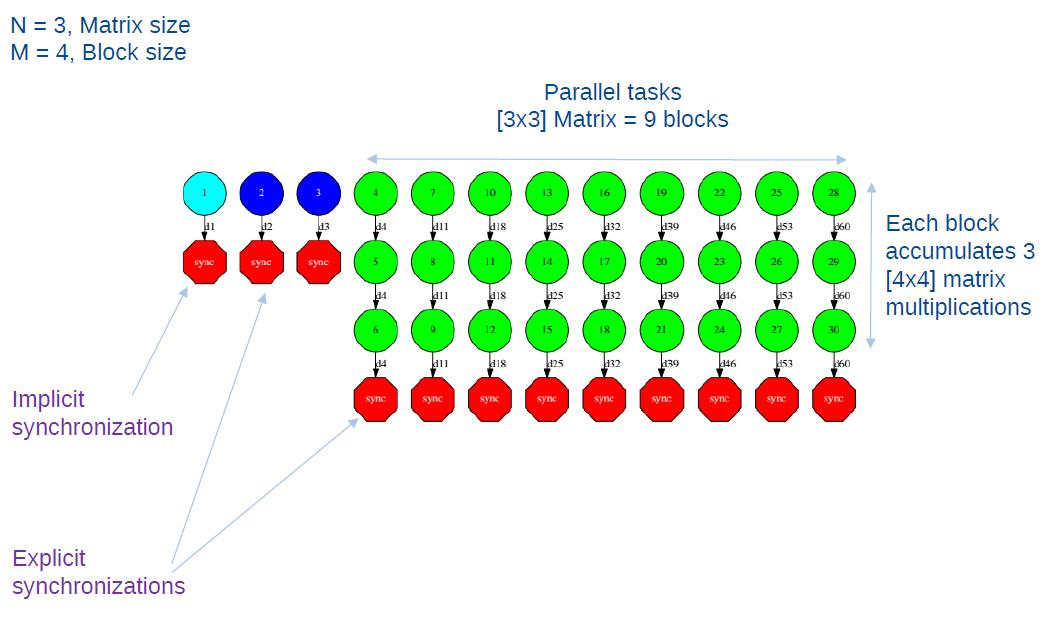
\includegraphics[width=1.0\textwidth]{./Sections/4_C/Figures/matmul.jpeg}
    \caption{Matmul Execution Graph.}
    \label{fig:matmul_exec_graph}
\end{figure}
